\chapter{Evaluation und Validation}
\label{ch:Eval}

\section{Vergleich mit Anforderungen}
\label{sec:VergleichAnforderungen}

\section{Fremde Wärmequellen}
\label{sec:FremdeWärmequellen}

In diesem Versuch wurde der Einfluss von fremden Wärmequellen wie zum Beispiel Laptops, Natels, oder Kaffees, Evaluiert. Dabei wurde der Effekt von Störquellen mit und ohne Personen im Raum analysiert.

\subsection{Resultate}
\label{subsec:FWresultate}

Der Threshold Algorithmus kann wie erwartet nicht gut mit anderen Wärmequellen umgehen. Dies weil der Threshold Algorithmus nur durch Temperatur und Mindestgrösse eines Objekts entscheiden Kann ob es sich um eine Person handelt. Deshalb hatte der Threshold Algorithmus auch eine nur eine Presicion score von \{Define\} erreicht.

Das CNN kann sehr gut mit anderen Wärmequellen umgehen, solange diese in ähnlicher Form antrainiert wurden. Da in einem Sitzungszimmer nicht viele unterschiedliche wärmequellen vorkommen.

\begin{figure}[h!]
	\begin{subfigure}{.3\linewidth}
		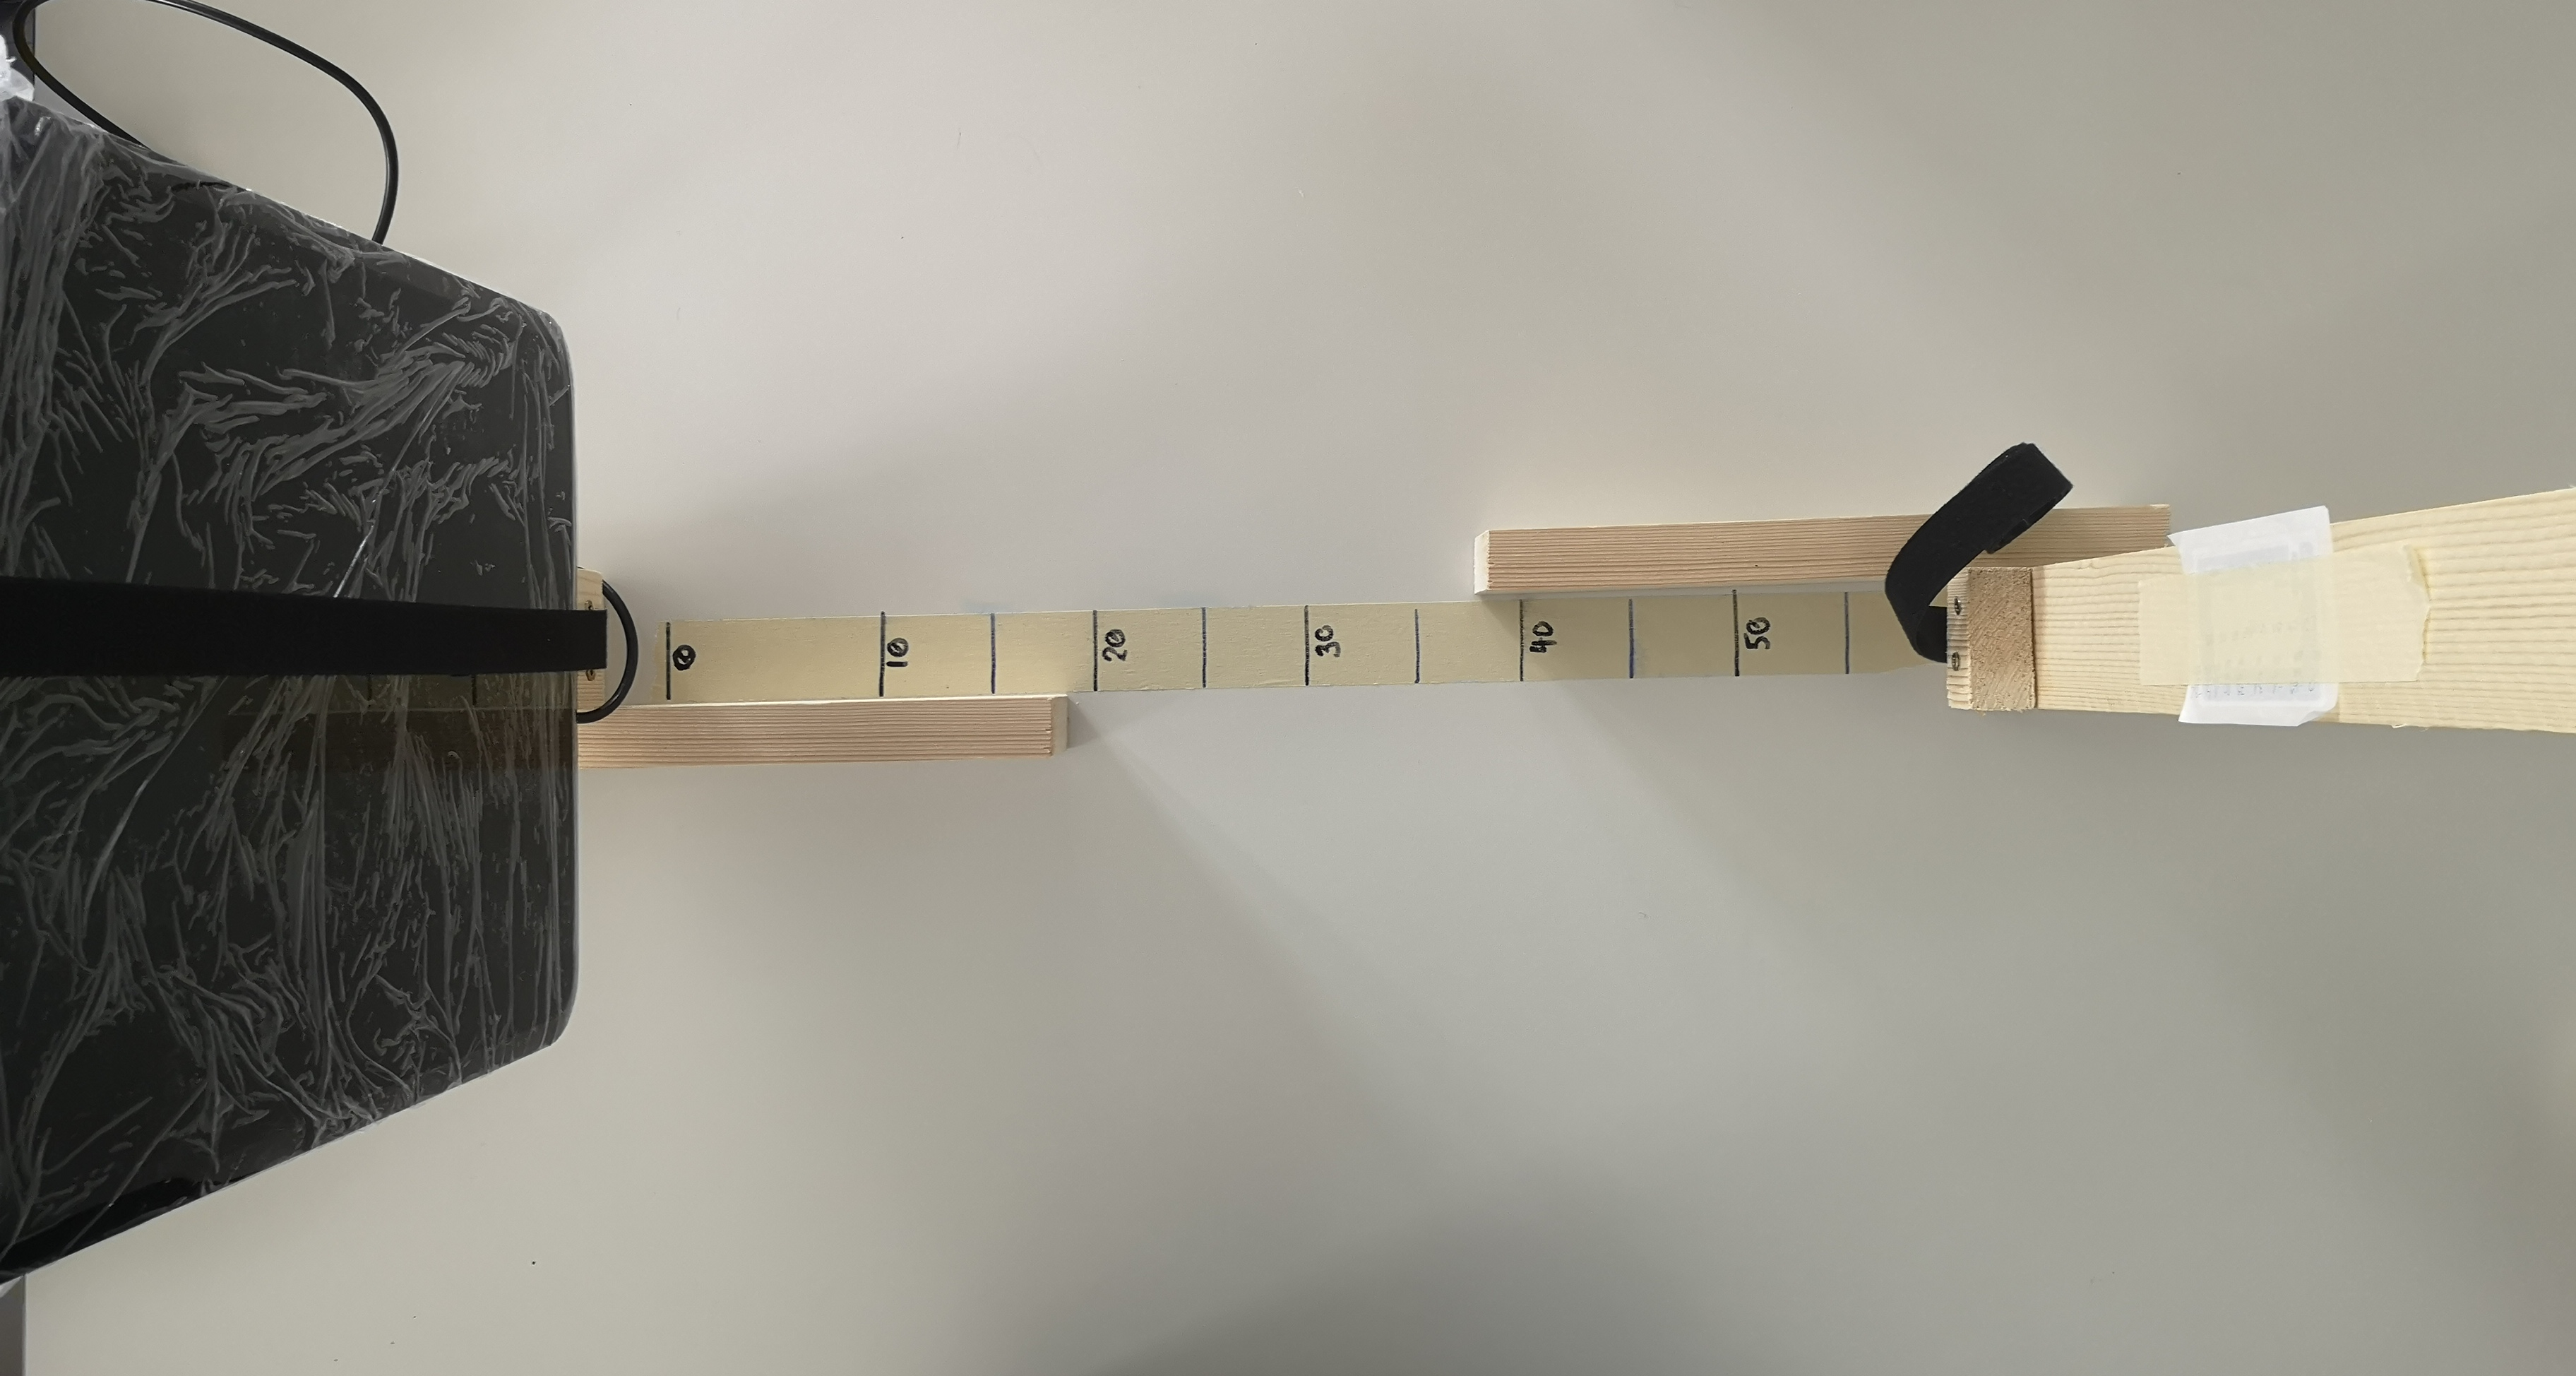
\includegraphics[keepaspectratio,height=4cm]{Versuch1MaximaleDistanz}
		\caption{Versuches Nummer 1 mit einem Abstand von 60cm}
		\label{fig:versuchaufbaunmr1}
	\end{subfigure}\hfill%
	\begin{subfigure}{.3\linewidth}
		\centering
		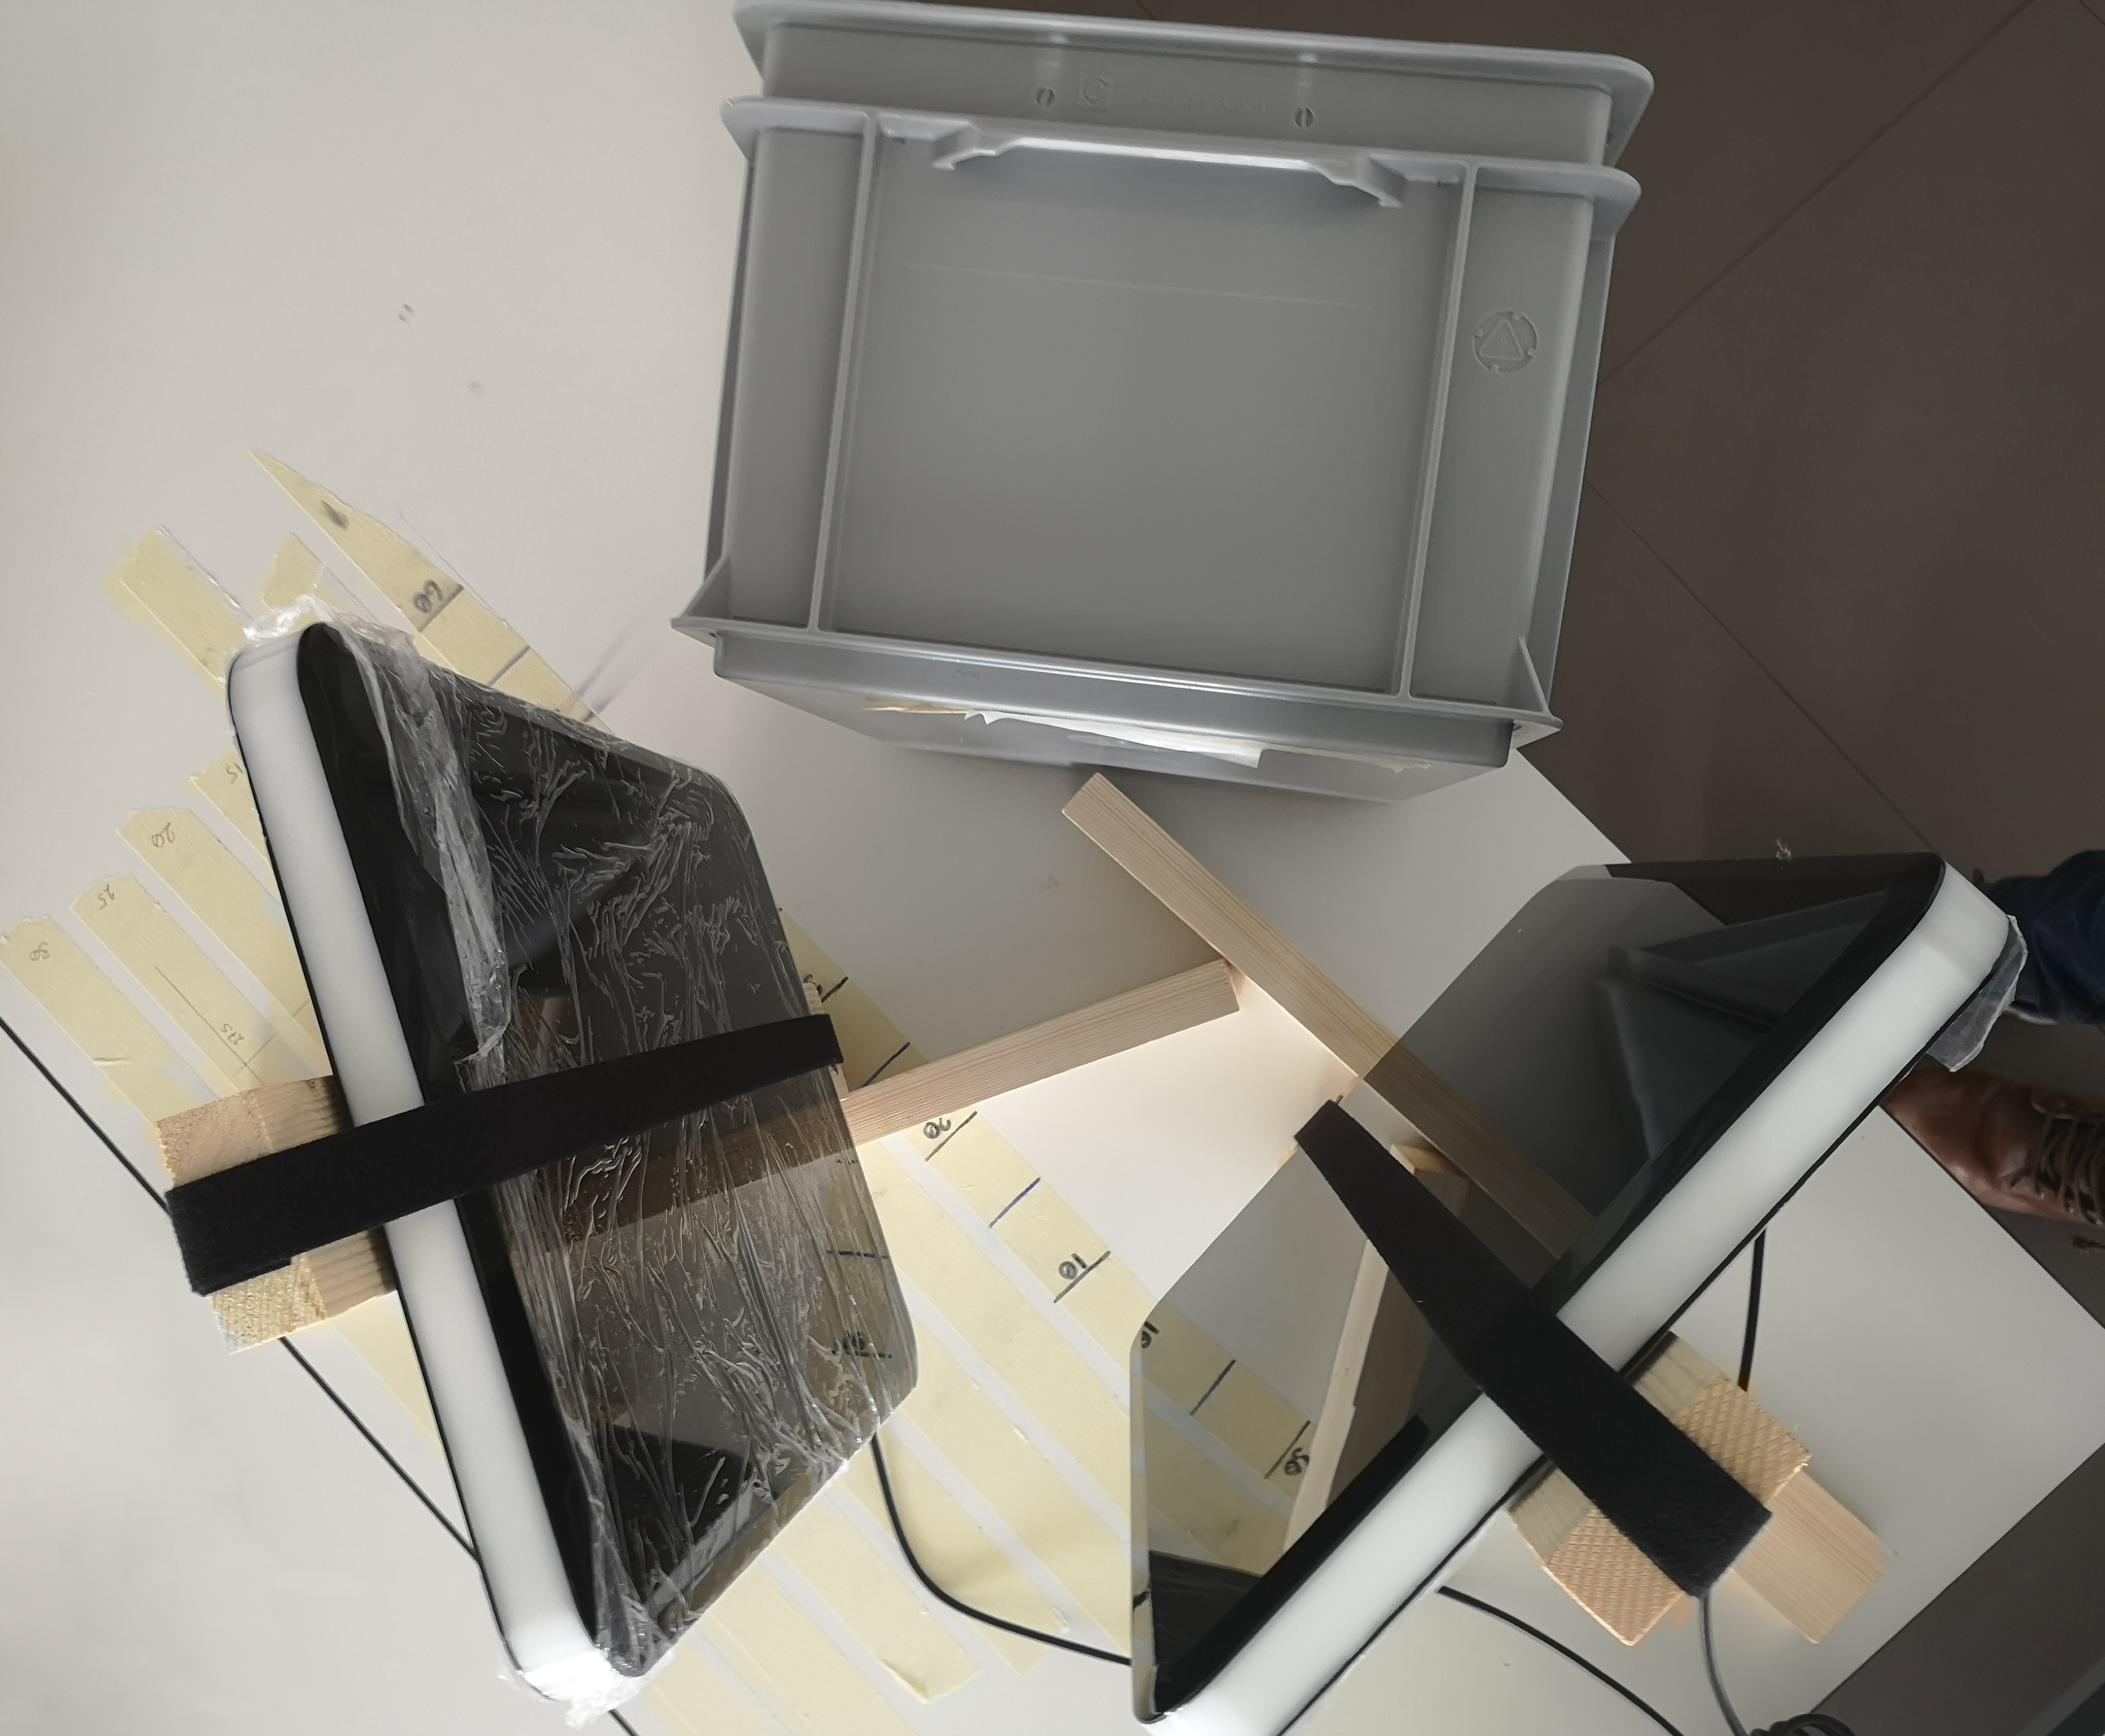
\includegraphics[keepaspectratio,height=4cm]{TestInterferenzAntennen}
		\caption{Versuch Nummer 7 mit einem Winkel von 60\SIUnitSymbolDegree}
		\label{fig:versuchaufbaunmr7}
	\end{subfigure}
\begin{subfigure}{.3\linewidth}
	\centering
	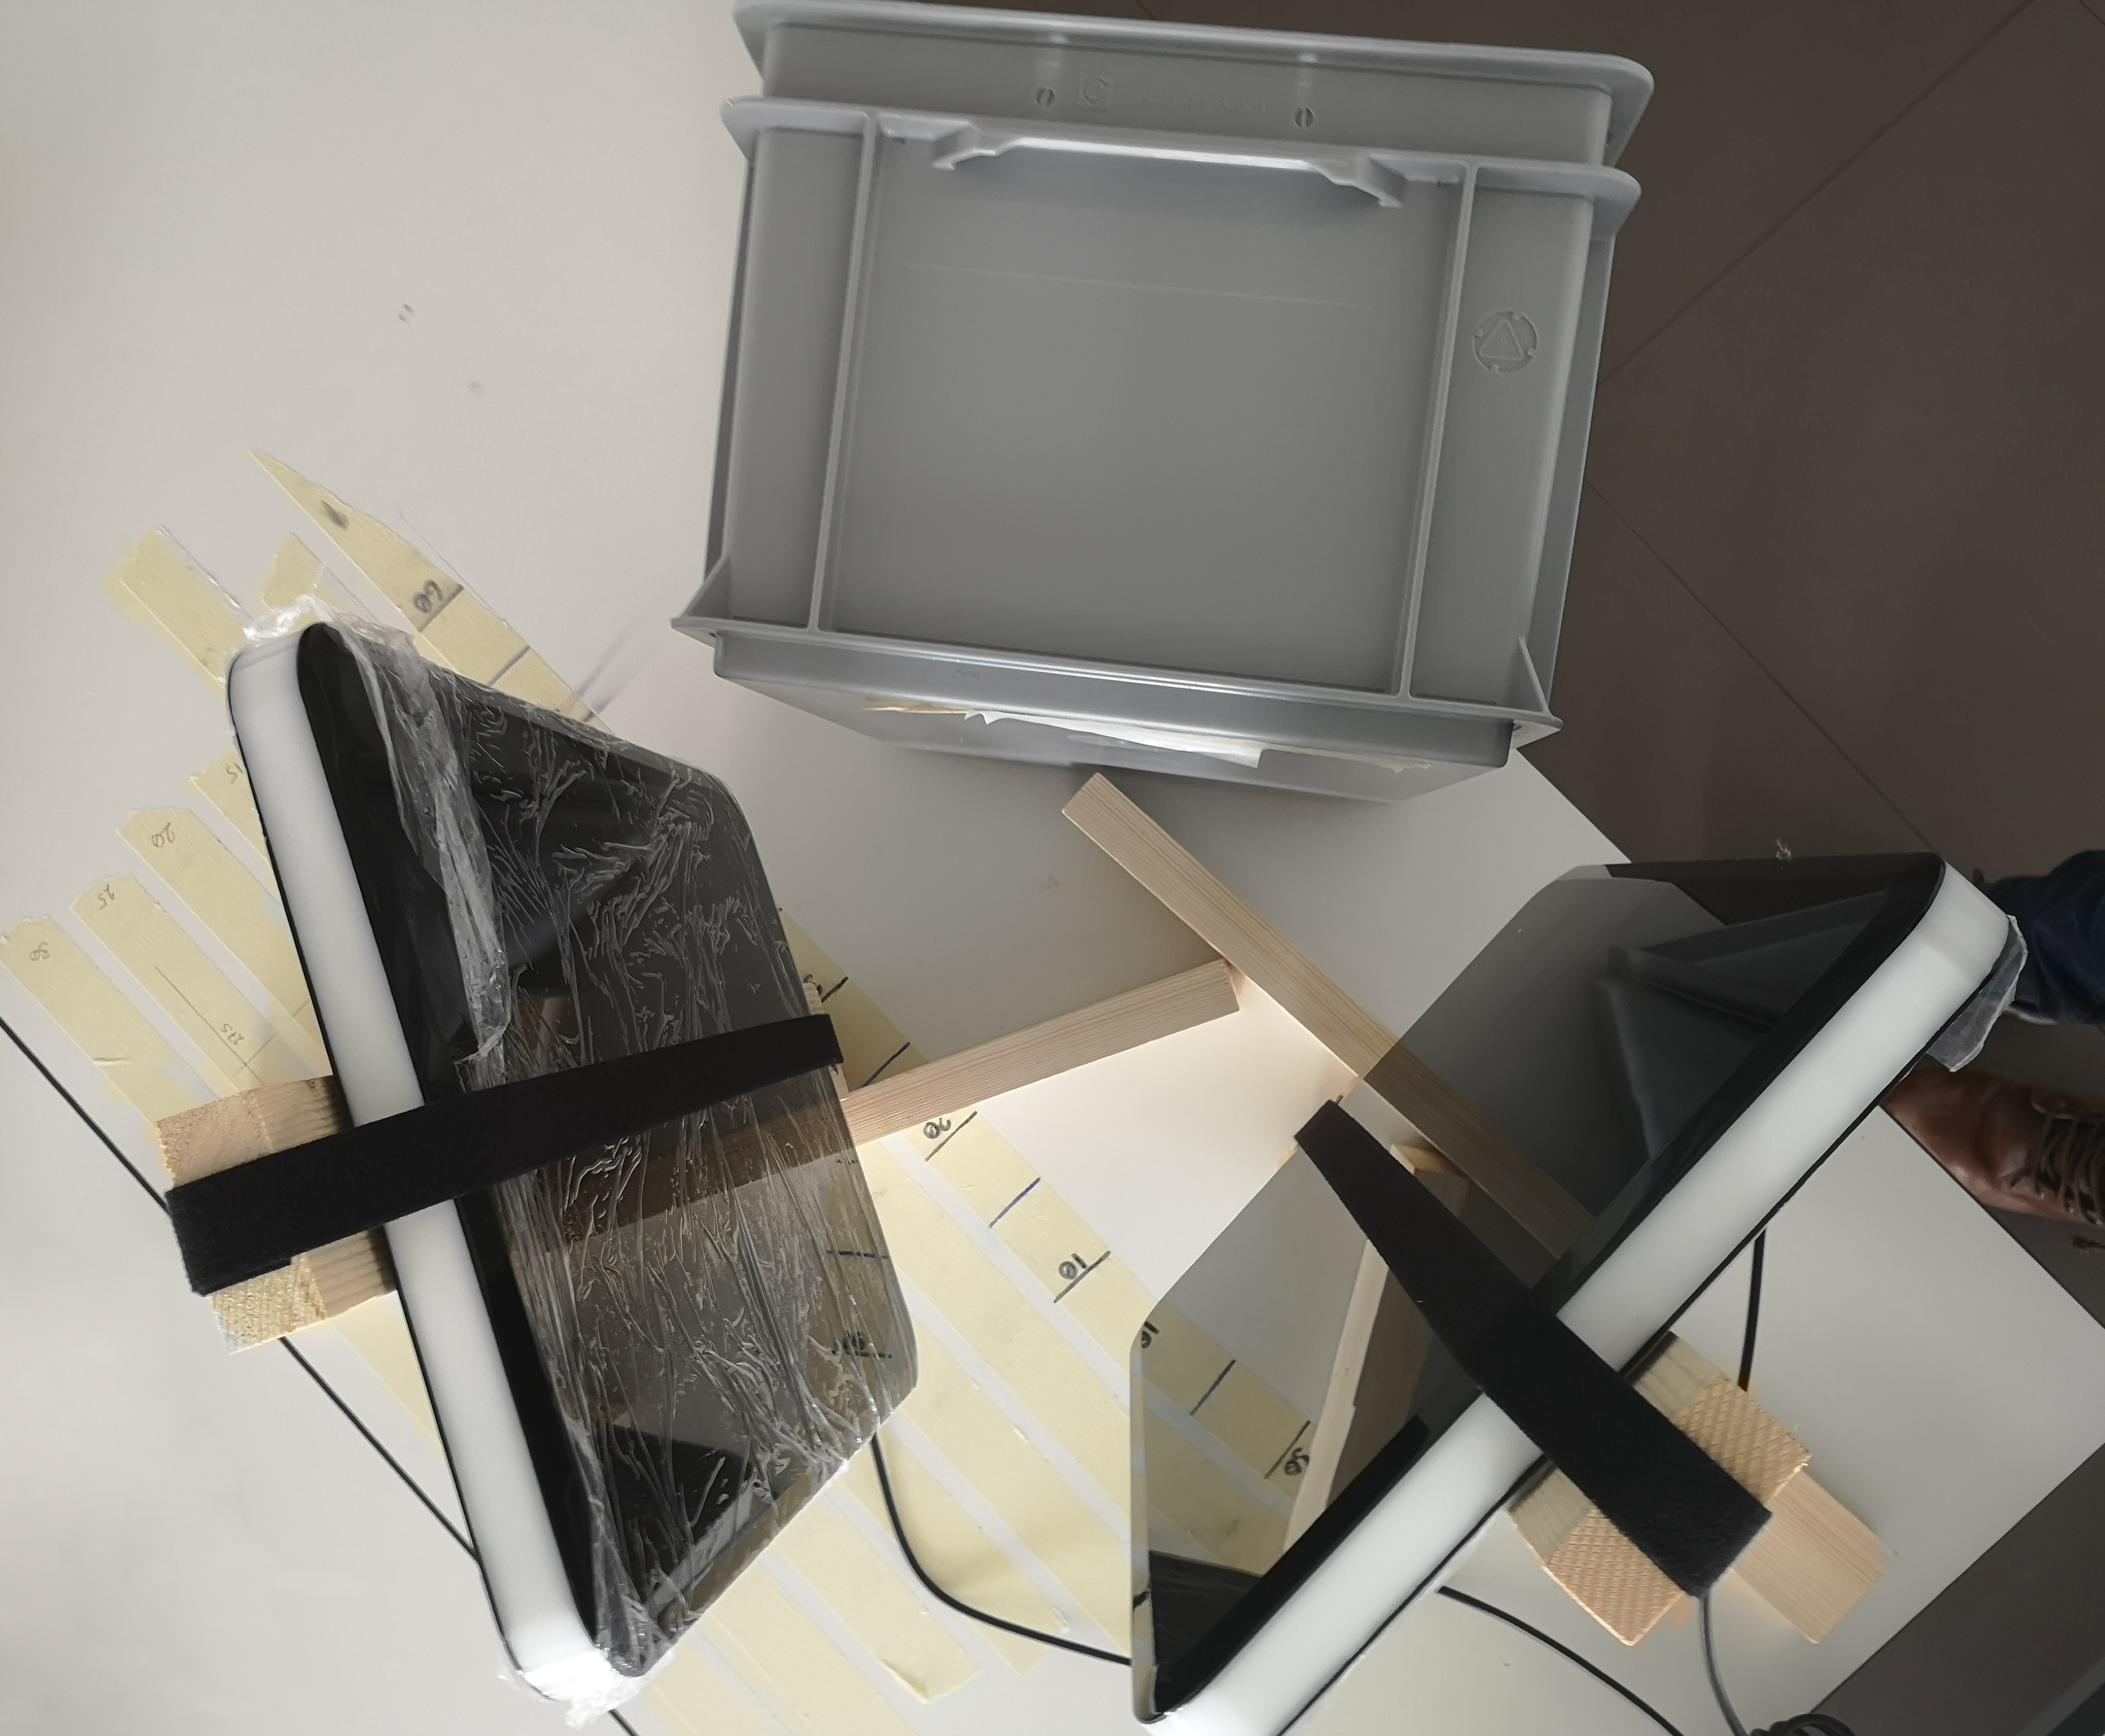
\includegraphics[keepaspectratio,height=4cm]{TestInterferenzAntennen}
	\caption{Versuch Nummer 7 mit einem Winkel von 60\SIUnitSymbolDegree}
	\label{fig:versuchaufbaunmr7}
\end{subfigure}
	\caption{Zwei Versuchsaufbauten}
	\label{fig:versuchsaufbauten}
\end{figure}
